\documentclass{article}
\usepackage{listings}
\usepackage{xcolor}
\usepackage{caption}
\usepackage{graphicx, subfig}
\usepackage{float}
\usepackage[utf8]{inputenc}
\usepackage{fontspec}
% \setmonofont{Sarasa-Mono-Slab-SC-Regular}

\lstset{
basicstyle=\ttfamily\scriptsize,
numbers=none,
breaklines,%自动换行
columns=flexible,%不随便添加空格,只在已经有空格的地方添加空格
keywordstyle=\color{blue}, %设置关键字颜色
        commentstyle=\color[cmyk]{1,0,1,0}, %设置注释颜色
numberstyle=\tiny,
frame=shadowbox,
rulesepcolor=\color{red!20!green!20!blue!20},
escapeinside=`', %将中文放在`和'之间,可以在lstlisting环境中准确的显示中文
}

\title{Assignment 2}
\author{Wangzhihui Mei, HongYi Huang, ChangXu, Zijia He}
\date{November 2020}

\begin{document}

\maketitle
\section{Task1}
\subsection{data describe}
Cardiovascular diseases (CVDs) is the leading cause of mortality in India. Ischemic heart disease and stroke are the predominant causes and are responsible for nearly 80\% of CVD deaths. 

\begin{lstlisting}[language=R]
dt <- read.csv("heart1.csv",na.strings = "?")
dt <- na.omit(dt) # handle NA
head(dt)
age sex cp trestbps chol fbs restecg thalach exang oldpeak slope ca thal target
1  63   1  3      145  233   1       0     150     0     2.3     0  0    1      1
2  37   1  2      130  250   0       1     187     0     3.5     0  0    2      1
3  41   0  1      130  204   0       0     172     0     1.4     2  0    2      1
4  56   1  1      120  236   0       1     178     0     0.8     2  0    2      1
5  57   0  0      120  354   0       1     163     1     0.6     2  0    2      1
6  57   1  0      140  192   0       1     148     0     0.4     1  0    1      1
\end{lstlisting} 
This database contains 14 attributes. The "target" field refers to the presence of CVD in the patient. It is
integer valued 0 (no presence) or 1 (presence). Next we look in detail at the data characteristics of each attribute.
\\
Age: Age in years\\
Sex: (1 = male; 0 = female)\\
CP:Chest pain type(1-typical angina, 2-atypical angina, 3-non-anginal	pain, 4-asymptomatic )\\
trestbps:Resting blood pressure (in mm Hg on admission to the hospital)\\
Chol:Serum cholestoral in mg/dl\\
Fbs:Indicator of whether fasting blood sugar>120 mg/dl (1-true; 0-false)\\
restecg:Resting electrocardiographic results\\
exang:Exercise induced angina (1-yes; 0-no)\\
oldpeak:ST depression induced by exercise relative to rest\\
slope:Slope of the peak exercise ST segment (1-upsloping, 2-flat, 3-downsloping)\\
ca:Number of major vessels (0-3) colored by flourosopy\\
thal:Summary of heart condition(3 = normal, 6 = fixed defect, 7=reversable defect)\\
target:the “The Disease Diagnosis” field refers to the presence of heart disease in the patient(0-No presence,1-Presence) 
\begin{lstlisting}[language=R]
<- summary(dt)
age        sex     cp         trestbps          chol       fbs     restecg    thalach      exang      oldpeak    
Min.   :29.00   0: 96   0:143   Min.   : 94.0   Min.   :126.0   0:258   0:147   Min.   : 71.0   0:204   Min.   :0.00  
1st Qu.:47.50   1:207   1: 50   1st Qu.:120.0   1st Qu.:211.0   1: 45   1:152   1st Qu.:133.5   1: 99   1st Qu.:0.00  
Median :55.00           2: 87   Median :130.0   Median :240.0           2:  4   Median :153.0           Median :0.80  
Mean   :54.37           3: 23   Mean   :131.6   Mean   :246.3                   Mean   :149.6           Mean   :1.04  
3rd Qu.:61.00                   3rd Qu.:140.0   3rd Qu.:274.5                   3rd Qu.:166.0           3rd Qu.:1.60  
Max.   :77.00                   Max.   :200.0   Max.   :564.0                   Max.   :202.0           Max.   :6.20  

slope         ca         thal        target      
0: 21   Min.   :0.0000   0:  2   Min.   :0.0000  
1:140   1st Qu.:0.0000   1: 18   1st Qu.:0.0000  
2:142   Median :0.0000   2:166   Median :1.0000  
        Mean   :0.7294   3:117   Mean   :0.5446  
        3rd Qu.:1.0000           3rd Qu.:1.0000  
        Max.   :4.0000           Max.   :1.0000  
\end{lstlisting}

\subsection{logistic regression}
By looking at the details of each data item in the dataset, it was found that the values of age as well as maximum heart rate were quite different and needed to be processed for both data items.
\begin{lstlisting}[language=R]
summary(dt$age)
dt$age<-cut(as.numeric(dt$age),breaks=3,labels=c("low1","normal1","high1"))
levels(dt$age)
table(dt$age)
> summary(dt$age)
   Min. 1st Qu.  Median    Mean 3rd Qu.    Max. 
  29.00   47.50   55.00   54.37   61.00   77.00 
> dt$age<-cut(as.numeric(dt$age),breaks = 3,labels=c("low1","normal1","high1"))
> levels(dt$age)
[1] "low1"    "normal1" "high1"  
> table(dt$age)

   low1 normal1   high1 
     64     168      71 
> summary(dt$chol)
Min. 1st Qu.  Median    Mean 3rd Qu.    Max. 
126.0   211.0   240.0   246.3   274.5   564.0 
> dt$chol<-cut(as.numeric(dt$chol),breaks =3,labels=c("low","normal","high"))
> levels(dt$chol)
[1] "low"    "normal" "high"  
> table(dt$chol)

low normal   high 
222     80      1 
\end{lstlisting}

Dividing the data set into training and test sets according to a 7 to 3 ratio
\begin{lstlisting}
  > samp<-sample(2,nrow(dt),replace = T,prob = c(0.7,0.3))
> training<-dt[samp==1,]
> test<-dt[samp==2,]
> head(training)
      age sex cp trestbps   chol fbs restecg thalach exang oldpeak slope ca thal target
1   high1   1  3      145    low   1       0     150     0     2.3     0  0    1      1
3    low1   0  1      130    low   0       0     172     0     1.4     2  0    2      1
4 normal1   1  1      120    low   0       1     178     0     0.8     2  0    2      1
5 normal1   0  0      120 normal   0       1     163     1     0.6     2  0    2      1
6 normal1   1  0      140    low   0       1     148     0     0.4     1  0    1      1
7 normal1   0  1      140 normal   0       0     153     0     1.3     1  0    2      1
> head(test)
       age sex cp trestbps   chol fbs restecg thalach exang oldpeak slope ca thal target
2     low1   1  2      130    low   0       1     187     0     3.5     0  0    2      1
18   high1   0  3      150    low   0       1     114     0     2.6     0  0    2      1
25    low1   1  3      140    low   0       1     178     1     1.4     2  0    3      1
29   high1   0  2      140 normal   1       0     157     0     0.8     2  1    2      1
36 normal1   0  2      142    low   0       0     160     1     1.4     0  0    2      1
38 normal1   1  2      150    low   0       0     165     0     1.6     2  0    3      1
> colSums(is.na(test))
     age      sex       cp trestbps     chol      fbs  restecg  thalach    exang  oldpeak    slope       ca     thal   target 
       0        0        0        0        0        0        0        0        0        0        0        0        0        0 
\end{lstlisting}

Next, a logistic regression prediction model is built using the training set data

\begin{lstlisting}[language=R]
> mod<-glm(target~.,data = training,family = binomial('logit'))
> summary(mod)

Call:
glm(formula = target ~ ., family = binomial("logit"), data = training)

Deviance Residuals: 
    Min       1Q   Median       3Q      Max  
-2.6397  -0.3260   0.1472   0.4614   2.4521  

Coefficients:
              Estimate Std. Error z value Pr(>|z|)   
(Intercept)    1.43597    3.14892   0.456  0.64838   
agenormal1    -1.08551    0.66165  -1.641  0.10088   
agehigh1       0.19073    0.82340   0.232  0.81682   
sex1          -1.27014    0.63533  -1.999  0.04559 * 
cp1            1.07789    0.64981   1.659  0.09716 . 
cp2            1.76202    0.59697   2.952  0.00316 **
cp3            2.33462    0.87380   2.672  0.00754 **
trestbps      -0.02011    0.01359  -1.480  0.13899   
cholnormal    -0.87024    0.56281  -1.546  0.12204   
cholhigh      13.46342 1455.39800   0.009  0.99262   
fbs1           1.40058    0.78331   1.788  0.07377 . 
restecg1       0.75994    0.47349   1.605  0.10850   
restecg2       0.18667    3.24270   0.058  0.95409   
thalach        0.01516    0.01288   1.177  0.23910   
exang1        -1.06170    0.53172  -1.997  0.04585 * 
oldpeak       -0.52696    0.26619  -1.980  0.04774 * 
slope1        -0.74014    1.04764  -0.706  0.47989   
slope2         0.01442    1.13336   0.013  0.98985   
ca            -0.57276    0.23372  -2.451  0.01426 * 
thal1          1.48527    2.16992   0.684  0.49367   
thal2          1.70341    1.83567   0.928  0.35343   
thal3          0.18380    1.87081   0.098  0.92174   
---
Signif. codes:  0 ‘***’ 0.001 ‘**’ 0.01 ‘*’ 0.05 ‘.’ 0.1 ‘ ’ 1

(Dispersion parameter for binomial family taken to be 1)

    Null deviance: 292.99  on 213  degrees of freedom
Residual deviance: 134.65  on 192  degrees of freedom
AIC: 178.65

Number of Fisher Scoring iterations: 14
\end{lstlisting} 
After getting the training model, we need to evaluate the suitability of the model for the scenario by the following metrics
\begin{lstlisting}[language=R]
  predicted<-predict(mod,training,type ="response")
  training$predd<-round(predicted,3)
  View(training)
  ggplot( training, aes( training$predd, color = as.factor(training$target) ) ) + 
    geom_density( ) +
    ggtitle( "Training Set's Predicted Score" )
  training$predw<-ifelse(training$predd>0.46,1,0)
\end{lstlisting}
\begin{figure}[H]
  \centering
  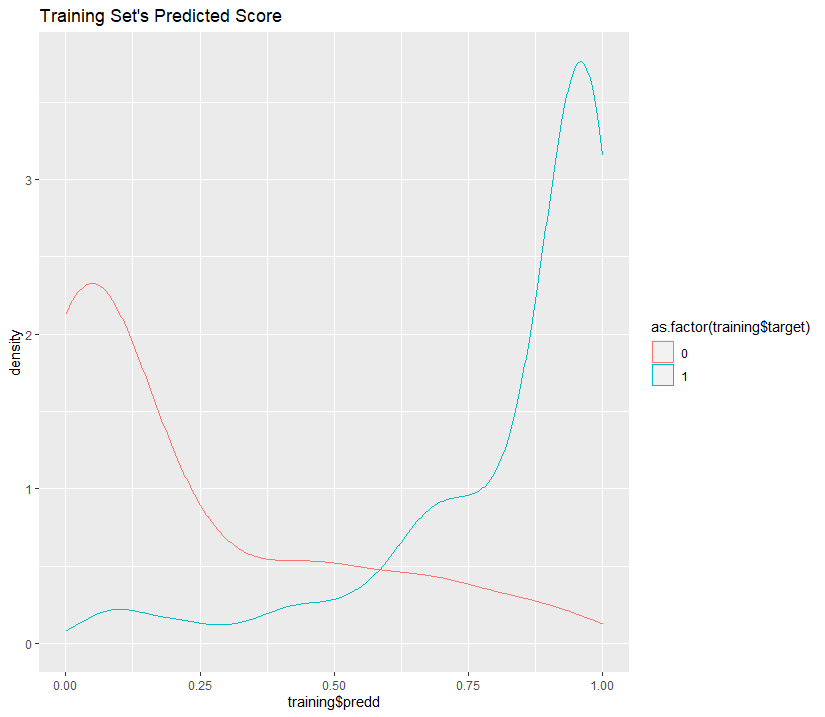
\includegraphics[width=1\textwidth]{1_1_trainScore.png}
\end{figure}

\begin{lstlisting}
> training$predw<-ifelse(training$predd>0.46,1,0)
> confusn<-confusionMatrix(training$target,training$predw,threshold = 0.46)
> confusn
   0   1
0 74  11
1 19 110
> confusn<-as.matrix(confusn)
> AccuracyRate <- sum(diag(confusn))/sum(confusn)
> AccuracyRate
[1] 0.8598131
\end{lstlisting}
Similarly, we need to evaluate this model in the test set
\begin{lstlisting}
> test$prob <- predict(mod,test,type = "response")
> View(test)
> ggplot( test, aes( test$prob, color = as.factor(test$target) ) ) + geom_density( size = 1 ) + ggtitle( "Test Set's Predicted Score" )
> test$predc<-ifelse(test$prob>0.475,1,0)
> confusn<-confusionMatrix(test$target,test$predc,threshold = 0.475)
> confusn
   0  1
0 31  7
1 14 37
> class(confusn)
[1] "data.frame"
> confusn<-as.matrix(confusn)
> AccuracyRate <- sum(diag(confusn))/sum(confusn)
> AccuracyRate
[1] 0.7640449
\end{lstlisting}
\begin{figure}[H]
  \centering
  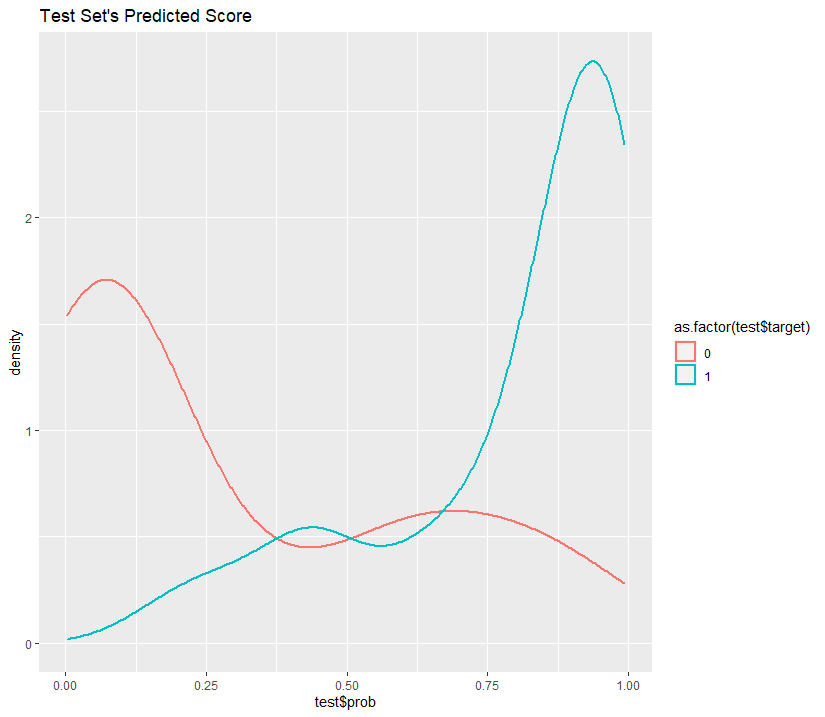
\includegraphics[width=1\textwidth]{1_1_testScore.png}
\end{figure}
The evaluation summary of logistic regression can be seen below
\begin{lstlisting}
  > Confusion
         Actual
Predicted  0  1
        0 31  7
        1 14 37
> AccuracyRate
[1] 0.7640449
> plot(rocCurve)
> rocCurve$sensitivities
[1] 1.0000000 0.6888889 0.0000000
> rocCurve$specificities
[1] 0.0000000 0.8409091 1.0000000
> rocCurve$au
Area under the curve: 0.7649
\end{lstlisting}

\subsection{Decision Tree}
The decision tree algorithm is a method of approximating the value of a discrete function. It is a typical classification method. It first processes the data, uses induction algorithms to generate readable rules and decision trees, and then uses decisions to analyze new data. In essence, a decision tree is a process of classifying data through a series of rules.

The decision tree algorithm constructs a decision tree to discover the classification rules contained in the data. How to construct a high-precision, small-scale decision tree is the core content of the decision tree algorithm. The decision tree construction can be done in two steps. The first step is to generate a decision tree: the process of generating a decision tree from the training sample set. In general, the training sample data set is a data set that has a history and a certain degree of comprehensiveness according to actual needs, and is used for data analysis and processing. The second step, the pruning of the decision tree: The pruning of the decision tree is the process of testing, correcting and pruning the decision tree generated in the previous stage, mainly using a new sample data set (called a test data set) The data verifies the preliminary rules generated during the decision tree generation process, and prunes those branches that affect the accuracy of the pre-balance.

We divided the original data set into two parts, using two-thirds of the data as the training set and the other third as the test set.
\begin{lstlisting}
> data<-read.csv("./heart.csv", head = TRUE, fileEncoding = 'GBK')
> set.seed(1)
> sub<-sample(1:nrow(data),round(nrow(data)*2/3))
> data_train<-data[sub,]
> data_test<-data[-sub,]
> dim(data_train)
[1] 202  14
> dim(data_test) 
[1] 101  14
\end{lstlisting}
Then we build a decision tree model and evaluate the model.
\begin{lstlisting}
> library(rpart)
> dt_model = rpart(target~., data = data_train,method = "class",parms = list(split="information"))
> summary(dt_model)
Call:
rpart(formula = target ~ ., data = data_train, method = "class", 
    parms = list(split = "information"))
  n= 202 

          CP nsplit rel error    xerror       xstd
1 0.50000000      0 1.0000000 1.0000000 0.07541752
2 0.05319149      1 0.5000000 0.5000000 0.06388682
3 0.04255319      3 0.3936170 0.5000000 0.06388682
4 0.01773050      4 0.3510638 0.5000000 0.06388682
5 0.01595745      7 0.2978723 0.5212766 0.06480973
6 0.01000000      9 0.2659574 0.5212766 0.06480973

Variable importance
      cp  thalach     thal    exang  oldpeak   age      sex    slope     chol       ca trestbps 
      21       18       15       11        8        7        7        5        3        3        3 

Node number 1: 202 observations,    complexity param=0.5
  predicted class=1  expected loss=0.4653465  P(node) =1
    class counts:    94   108
   probabilities: 0.465 0.535 
  left son=2 (95 obs) right son=3 (107 obs)
  Primary splits:
      cp    < 0.5   to the left,  improve=30.14774, (0 missing)
      thal  < 2.5   to the right, improve=25.50801, (0 missing)
      exang < 0.5   to the right, improve=21.12757, (0 missing)
      slope < 1.5   to the left,  improve=15.34173, (0 missing)
      ca    < 0.5   to the right, improve=14.98973, (0 missing)
  Surrogate splits:
      exang   < 0.5   to the right, agree=0.748, adj=0.463, (0 split)
      thalach < 143.5 to the left,  agree=0.703, adj=0.368, (0 split)
      thal    < 2.5   to the right, agree=0.663, adj=0.284, (0 split)
      oldpeak < 1.85  to the right, agree=0.624, adj=0.200, (0 split)
      slope   < 1.5   to the left,  agree=0.624, adj=0.200, (0 split)

Node number 2: 95 observations,    complexity param=0.05319149
  predicted class=0  expected loss=0.2526316  P(node) =0.470297
    class counts:    71    24
   probabilities: 0.747 0.253 
  left son=4 (54 obs) right son=5 (41 obs)
  Primary splits:
      thal    < 2.5   to the right, improve=13.701710, (0 missing)
      ca      < 0.5   to the right, improve= 7.720223, (0 missing)
      exang   < 0.5   to the right, improve= 7.709513, (0 missing)
      sex     < 0.5   to the right, improve= 6.603312, (0 missing)
      oldpeak < 0.7   to the right, improve= 6.334665, (0 missing)
  Surrogate splits:
      sex      < 0.5   to the right, agree=0.705, adj=0.317, (0 split)
      trestbps < 116   to the right, agree=0.674, adj=0.244, (0 split)
      exang    < 0.5   to the right, agree=0.642, adj=0.171, (0 split)
      oldpeak  < 0.05  to the right, agree=0.632, adj=0.146, (0 split)
      age   < 61.5  to the left,  agree=0.621, adj=0.122, (0 split)

Node number 3: 107 observations,    complexity param=0.0177305
  predicted class=1  expected loss=0.2149533  P(node) =0.529703
    class counts:    23    84
   probabilities: 0.215 0.785 
  left son=6 (84 obs) right son=7 (23 obs)
  Primary splits:
      age  < 44.5  to the right, improve=6.378769, (0 missing)
      sex     < 0.5   to the right, improve=5.146720, (0 missing)
      slope   < 1.5   to the left,  improve=4.543258, (0 missing)
      oldpeak < 0.75  to the right, improve=4.230748, (0 missing)
      thal    < 2.5   to the right, improve=3.621652, (0 missing)
  Surrogate splits:
      thalach < 181   to the left,  agree=0.841, adj=0.261, (0 split)

Node number 4: 54 observations
  predicted class=0  expected loss=0.05555556  P(node) =0.2673267
    class counts:    51     3
   probabilities: 0.944 0.056 

Node number 5: 41 observations,    complexity param=0.05319149
  predicted class=1  expected loss=0.4878049  P(node) =0.2029703
    class counts:    20    21
   probabilities: 0.488 0.512 
  left son=10 (9 obs) right son=11 (32 obs)
  Primary splits:
      thalach < 120   to the left,  improve=7.815108, (0 missing)
      ca      < 0.5   to the right, improve=6.988807, (0 missing)
      exang   < 0.5   to the right, improve=5.670943, (0 missing)
      slope   < 1.5   to the left,  improve=3.074021, (0 missing)
      sex     < 0.5   to the right, improve=2.822754, (0 missing)
  Surrogate splits:
      oldpeak < 3.1   to the right, agree=0.805, adj=0.111, (0 split)

Node number 6: 84 observations,    complexity param=0.0177305
  predicted class=1  expected loss=0.2738095  P(node) =0.4158416
    class counts:    23    61
   probabilities: 0.274 0.726 
  left son=12 (54 obs) right son=13 (30 obs)
  Primary splits:
      sex     < 0.5   to the right, improve=5.875620, (0 missing)
      slope   < 1.5   to the left,  improve=3.827789, (0 missing)
      oldpeak < 0.7   to the right, improve=2.782247, (0 missing)
      age  < 56.5  to the right, improve=2.433472, (0 missing)
      thal    < 2.5   to the right, improve=2.361801, (0 missing)
  Surrogate splits:
      chol    < 282.5 to the left,  agree=0.75, adj=0.300, (0 split)
      age  < 64.5  to the left,  agree=0.69, adj=0.133, (0 split)
      thalach < 118   to the right, agree=0.69, adj=0.133, (0 split)

Node number 7: 23 observations
  predicted class=1  expected loss=0  P(node) =0.1138614
    class counts:     0    23
   probabilities: 0.000 1.000 

Node number 10: 9 observations
  predicted class=0  expected loss=0  P(node) =0.04455446
    class counts:     9     0
   probabilities: 1.000 0.000 

Node number 11: 32 observations,    complexity param=0.04255319
  predicted class=1  expected loss=0.34375  P(node) =0.1584158
    class counts:    11    21
   probabilities: 0.344 0.656 
  left son=22 (10 obs) right son=23 (22 obs)
  Primary splits:
      ca      < 0.5   to the right, improve=4.0520220, (0 missing)
      exang   < 0.5   to the right, improve=3.1562630, (0 missing)
      sex     < 0.5   to the right, improve=1.3529580, (0 missing)
      chol    < 280.5 to the right, improve=0.9875400, (0 missing)
      thalach < 133.5 to the right, improve=0.8956238, (0 missing)
  Surrogate splits:
      chol    < 280.5 to the right, agree=0.844, adj=0.5, (0 split)
      age  < 66.5  to the right, agree=0.750, adj=0.2, (0 split)
      oldpeak < 1.8   to the right, agree=0.719, adj=0.1, (0 split)

Node number 12: 54 observations,    complexity param=0.0177305
  predicted class=1  expected loss=0.3888889  P(node) =0.2673267
    class counts:    21    33
   probabilities: 0.389 0.611 
  left son=24 (9 obs) right son=25 (45 obs)
  Primary splits:
      thalach < 135.5 to the left,  improve=3.418656, (0 missing)
      oldpeak < 0.7   to the right, improve=3.235388, (0 missing)
      age  < 56.5  to the right, improve=2.703478, (0 missing)
      chol    < 273.5 to the right, improve=2.543589, (0 missing)
      fbs     < 0.5   to the left,  improve=2.077240, (0 missing)
  Surrogate splits:
      chol < 180   to the left,  agree=0.870, adj=0.222, (0 split)
      thal < 1.5   to the left,  agree=0.852, adj=0.111, (0 split)

Node number 13: 30 observations
  predicted class=1  expected loss=0.06666667  P(node) =0.1485149
    class counts:     2    28
   probabilities: 0.067 0.933 

Node number 22: 10 observations
  predicted class=0  expected loss=0.3  P(node) =0.04950495
    class counts:     7     3
   probabilities: 0.700 0.300 

Node number 23: 22 observations
  predicted class=1  expected loss=0.1818182  P(node) =0.1089109
    class counts:     4    18
   probabilities: 0.182 0.818 

Node number 24: 9 observations
  predicted class=0  expected loss=0.2222222  P(node) =0.04455446
    class counts:     7     2
   probabilities: 0.778 0.222 

Node number 25: 45 observations,    complexity param=0.01595745
  predicted class=1  expected loss=0.3111111  P(node) =0.2227723
    class counts:    14    31
   probabilities: 0.311 0.689 
  left son=50 (25 obs) right son=51 (20 obs)
  Primary splits:
      oldpeak  < 0.55  to the right, improve=2.296979, (0 missing)
      age   < 56.5  to the right, improve=2.114354, (0 missing)
      trestbps < 131   to the right, improve=1.626569, (0 missing)
      chol     < 223.5 to the right, improve=1.539977, (0 missing)
      fbs      < 0.5   to the left,  improve=1.467395, (0 missing)
  Surrogate splits:
      slope    < 1.5   to the left,  agree=0.756, adj=0.45, (0 split)
      age   < 57.5  to the right, agree=0.689, adj=0.30, (0 split)
      cp       < 1.5   to the right, agree=0.644, adj=0.20, (0 split)
      trestbps < 131   to the right, agree=0.622, adj=0.15, (0 split)
      chol     < 223.5 to the right, agree=0.600, adj=0.10, (0 split)

Node number 50: 25 observations,    complexity param=0.01595745
  predicted class=1  expected loss=0.44  P(node) =0.1237624
    class counts:    11    14
   probabilities: 0.440 0.560 
  left son=100 (11 obs) right son=101 (14 obs)
  Primary splits:
      thalach  < 159   to the right, improve=1.5621710, (0 missing)
      trestbps < 131   to the right, improve=1.1420530, (0 missing)
      fbs      < 0.5   to the left,  improve=0.8954905, (0 missing)
      ca       < 0.5   to the right, improve=0.8185171, (0 missing)
      chol     < 236.5 to the left,  improve=0.6757523, (0 missing)
  Surrogate splits:
      age   < 58.5  to the left,  agree=0.76, adj=0.455, (0 split)
      trestbps < 139   to the left,  agree=0.68, adj=0.273, (0 split)
      chol     < 279.5 to the right, agree=0.68, adj=0.273, (0 split)
      cp       < 1.5   to the left,  agree=0.64, adj=0.182, (0 split)
      ca       < 0.5   to the right, agree=0.64, adj=0.182, (0 split)

Node number 51: 20 observations
  predicted class=1  expected loss=0.15  P(node) =0.0990099
    class counts:     3    17
   probabilities: 0.150 0.850 

Node number 100: 11 observations
  predicted class=0  expected loss=0.3636364  P(node) =0.05445545
    class counts:     7     4
   probabilities: 0.636 0.364 

Node number 101: 14 observations
  predicted class=1  expected loss=0.2857143  P(node) =0.06930693
    class counts:     4    10
   probabilities: 0.286 0.714 
\end{lstlisting}
Draw the decision tree.
\begin{lstlisting}
> library(rpart.plot)
> rpart.plot(dt_model)
\end{lstlisting}
 \begin{figure}[H]
\centering
  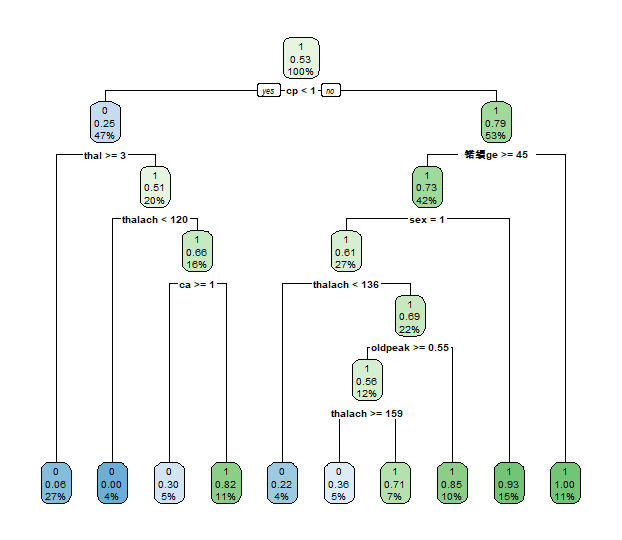
\includegraphics[width=.8\textwidth]{1-2-1.png} %1.png是图片文件的相对路径
\end{figure}
Using the trained model to predict the test data.
\begin{lstlisting}
> test_predict=predict(dt_model,newdata = data_test,type="class")
> test_predict
  3   4   5   6   7   8  10  11  12  18  21  23  32  35  38  46  47  52  54  55  58  59  62  63  66  67  68  69  74  76  81  82  91  94  95  96  97 
  1   0   1   1   1   1   0   1   1   1   0   1   0   0   0   1   1   1   1   1   1   1   1   1   1   1   1   1   1   1   1   1   1   1   1   0   1 
101 109 112 114 119 120 123 125 128 132 134 142 146 148 153 154 155 157 161 164 166 168 169 171 177 179 182 183 188 199 200 203 205 207 208 209 210 
  1   1   1   0   1   1   1   1   1   1   1   1   1   1   1   1   1   1   1   1   0   0   0   1   0   0   0   1   0   0   0   0   0   0   0   1   0 
212 214 215 216 219 229 235 238 241 243 249 250 251 260 264 266 272 276 278 280 281 288 289 295 296 298 303 
  0   0   0   0   0   1   0   0   0   0   1   1   0   1   0   0   1   0   1   0   1   1   0   1   0   0   1 
Levels: 0 1
> test_confusion=table(test_predict, data_test$target, dnn = c("Predicted", "Actual"))
> test_confusion
         Actual
Predicted  0  1
        0 31  8
        1 13 49
> acc <- sum(diag(test_confusion)) / sum(test_confusion)
> acc
[1] 0.7920792
\end{lstlisting}
Draw the ROC curve and calculate the AUC.
\begin{lstlisting}
> library(ROCR)
> test.pred<-prediction(test.predict[,2],data_test$target)
> test.perf<-performance(test.pred,"tpr","fpr")  
> View(test.perf) 
> plot(test.perf,main="ROC Curve",col = "blue", lty = 1, lwd = 3)
> auc_ROCR <- performance(test.pred, measure = "auc")
> auc_ROCR
A performance instance
  'Area under the ROC curve'
> auc_ROCR <- auc_ROCR@y.values[[1]]
> auc_ROCR
[1] 0.8598485
\end{lstlisting}
The AUC is 0.8598485.
 \begin{figure}[H]
\centering
  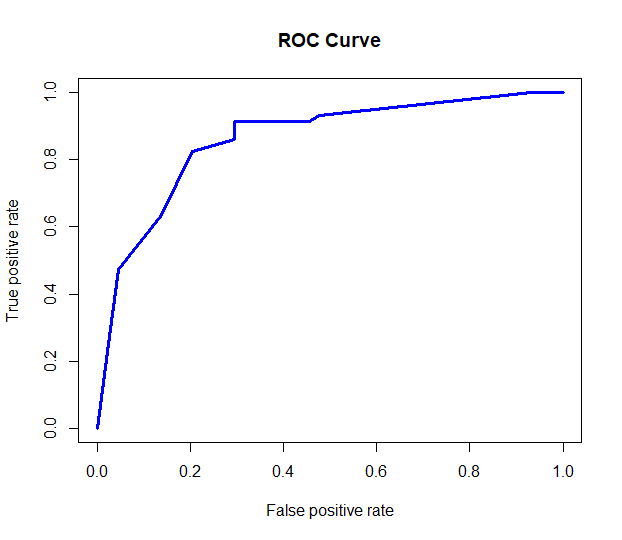
\includegraphics[width=.7\textwidth]{1-2-2.png} %1.png是图片文件的相对路径

\end{figure}


\subsection{Random Forest}
In machine learning, a random forest is a classifier containing multiple decision trees, and the output category is determined by the mode of the category output by the individual trees. Leo Breiman and Adele Cutler developed an algorithm to infer random forests. And "Random Forests" is their trademark. This term is derived from random decision forests proposed by Tin Kam Ho of Bell Labs in 1995. This method combines Breimans' "Bootstrap aggregating" idea and Ho's "random subspace method" to build a set of decision trees.

We divided the original data set into two parts, using two-thirds of the data as the training set and the other third as the test set.
\begin{lstlisting}
> data<-read.csv("./heart.csv", head = TRUE, fileEncoding = 'GBK')
> set.seed(1)
> sub<-sample(1:nrow(data),round(nrow(data)*2/3))
> data_train<-data[sub,]
> data_test<-data[-sub,]
> dim(data_train)
[1] 202  14
> dim(data_test) 
[1] 101  14
\end{lstlisting}
Constructing a random forest and see the importance of each attribute.
\begin{lstlisting}
> data_train$target = as.factor(data_train$target)
> data_test$target = as.factor(data_test$target)
> heart_randomforest <- randomForest(target ~ .,data = data_train,ntree =500,mtry=3,importance=TRUE ,proximity=TRUE)
> wine_randomforest$importance
> heart_randomforest$importance
                     0           1 MeanDecreaseAccuracy MeanDecreaseGini
age    0.0044937516 0.011962156         0.0086940003         8.478937
sex       0.0145044314 0.028124986         0.0218931544         4.485431
cp        0.0574064595 0.040003224         0.0477923304        14.602807
trestbps  0.0012780918 0.004201236         0.0027883228         7.904588
chol     -0.0042746775 0.004597818         0.0006192567         8.319724
fbs       0.0003928993 0.001395237         0.0009719512         1.478607
restecg   0.0021038577 0.001391102         0.0016794871         1.961444
thalach   0.0125979001 0.026459197         0.0200311648        11.766105
exang     0.0257168826 0.018111586         0.0217800801         7.691388
oldpeak   0.0174696577 0.009578546         0.0130692595         9.089572
slope     0.0138465158 0.009035109         0.0110925198         4.770929
ca        0.0144427976 0.025380724         0.0201100161         7.771338
thal      0.0363102817 0.043796083         0.0402148715        10.913105
> varImpPlot(heart_randomforest, main = "variable importance")
\end{lstlisting}
 \begin{figure}[H]
\centering
  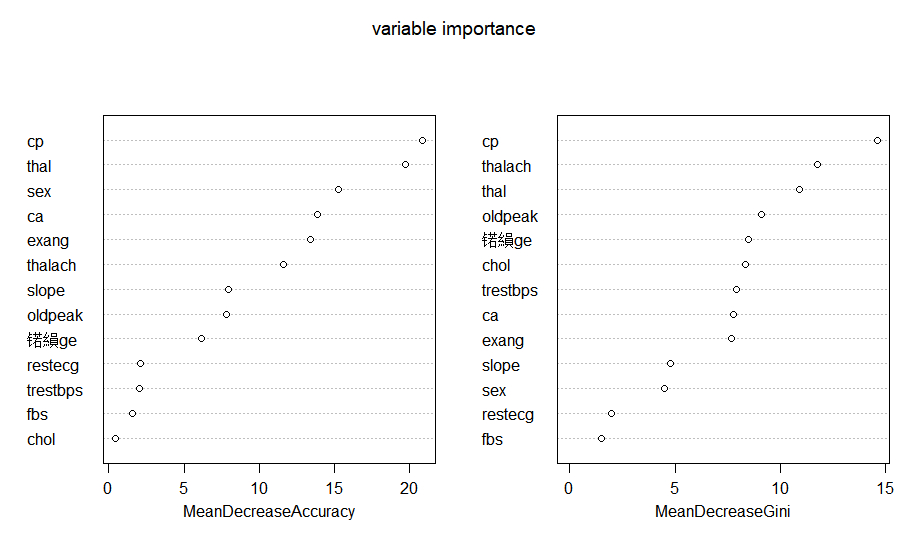
\includegraphics[width=1\textwidth]{1-3-1.png} %1.png是图片文件的相对路径

\end{figure}
Predicting test data with the trained model
\begin{lstlisting}
> pre_ran <- predict(heart_randomforest,newdata=data_test)
> obs_p_ran = data.frame(prob=pre_ran,obs=data_test$target)
> table(data_test$target,pre_ran,dnn=c("True","Predict"))
    Predict
True  0  1
   0 35  9
   1  7 50
> test_confusion=table(data_test$target,pre_ran,dnn=c("True","Predict"))
> acc <- sum(diag(test_confusion)) / sum(test_confusion)
> acc
[1] 0.8415842
\end{lstlisting}
ROC curve and AUC value
 \begin{figure}[H]
\centering
  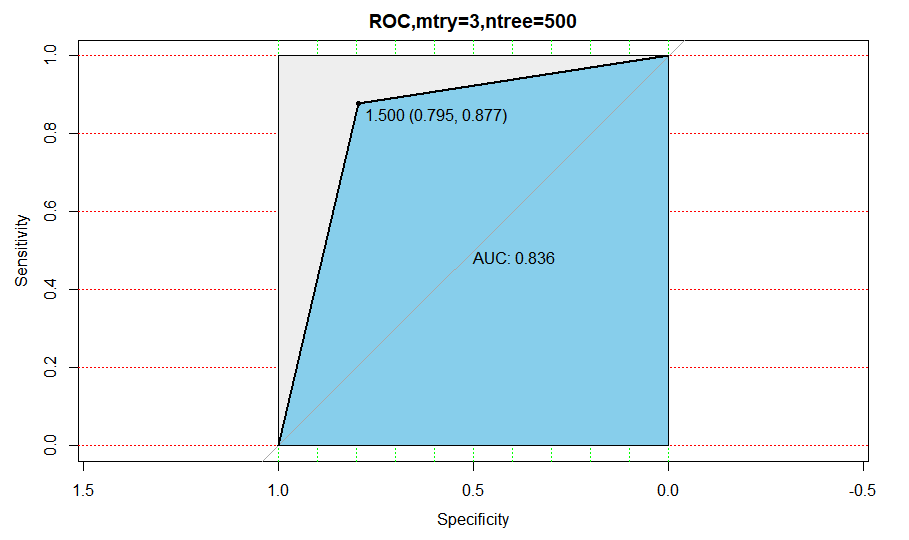
\includegraphics[width=1\textwidth]{1-3-2.png} %1.png是图片文件的相对路径
\end{figure}



\subsection{discuss}
\begin{table}[H]
  \centering
  \begin{tabular}{llll}
  Result    & Logistic Regression & Decision Tree & Random forest \\ \cline{2-4} 
  Accurancy & 0.764               & 0.792         & 0.841         \\ \cline{2-4} 
  AUC       & 0.765               & 0.859         & 0.836         \\ \cline{2-4} 
  \end{tabular}
\end{table}
For bicategorization problems logistic regression is a frequently used method, the logistic regression algorithm is to find a hyperplane in the sample data, which can then be accurately separated into categories and be able to classify the corresponding new data features.\\
The tree model is processed one feature at a time, before the linear model is where all features are given weights and summed to get a new value. The difference between decision tree and logistic regression is that logistic regression converts all the features into probability and divides them into one category if they are greater than a probability threshold and another category if they are less than a probability threshold, while decision tree divides each feature into one category. Also logistic regression can only find a linear partition (between input feature x and logit is linear, unless a multidimensional mapping of x is performed), while decision tree can find a non-linear partition.\\
The tree model is closer to the human mind, which can produce visual classification rules, and the resulting model is interpretable (can extract rules). The functions fitted by the tree model are actually step functions of the partitioning interval.\\
In spite of pruning and other methods, one tree is still definitely not as good as multiple trees, hence the random forest, which addresses the weakness of decision tree generalization.\\
Based on the predictions for this heart problem dataset, we can find that: \\
1. logistic regression is better at analyzing the overall structure of data than decision trees, while decision trees are better at analyzing the local structure than logistic regression.
(2) Logistic regression is good at analyzing linear relationships, while decision trees have a poor grasp of linear relationships. Although dealing with nonlinear relationships is the strength of decision trees, many nonlinear relationships can be approximated entirely by linear relationships and work well. Linear relationships have many advantages in practice: they are concise, easy to understand, and can prevent overfitting of the data to some extent.
3. logistic regression is sensitive and susceptible to extreme values, and decision trees perform better in this respect.
\section{Task2}
\subsection{Describe the Reuters-21578 corpus}
Reuters-21578 is a test collection for text classification research that is a multi-class, multi-label dataset. This dataset contains 90 classes, 7769 training files, and 3019 test files is a ModApte subdirectory of the Reuters-21578 benchmark. The Reuters-21578 dataset was originally collected and tagged by the Carnegie Group and Reuters in 1987 during the development of the CONSTRUE text classification system, and later by AT\&T Labs Research in September 1997. released in February, with David D. Lewis as the lead publisher

\subsection{Describe how each document is represented in your implementation.}
\begin{lstlisting}[language=R]
> data(Reuters21578)
> class(Reuters21578)
[1] "VCorpus" "Corpus" 
> head(Reuters21578)
<<VCorpus>>
Metadata:  corpus specific: 0, document level (indexed): 0
Content:  documents: 6
> summary(Reuters21578)
      Length Class             Mode
1     2      PlainTextDocument list
2     2      PlainTextDocument list
3     2      PlainTextDocument list
4     2      PlainTextDocument list
5     2      PlainTextDocument list
...
\end{lstlisting}

We import the Reuters-21578 as Vcorpus, which contains Metadata and Content. The metadata attribute contains author, datetime stamp, description, heading id, language, origin, lewissplit, cgisplit, oldid, topics\_cat, places, people, orgs, exchanges. The content is the raw data.

The data structure in the tm package that mainly manages documents is called Corpus, which represents a collection of documents. The corpus is divided into a dynamic corpus (Volatile Corpus) and a static corpus (Permanent Corpus). A dynamic corpus will be stored in memory as an R object and can be generated by either VCorpus() or Corpus(). The dynamic corpus, on the other hand, is stored as an R external file and can be generated using the PCorpus() function.

\subsection{Describe the whole procedure on applying LDA to this corpus to perform topic modeling.}
\begin{enumerate}
  \item Import the dataset
  \item Pre-processing the dataset, including transforming the content to lower case, striping whitespace, removing stopwords, punctuation and numbers, and steming document. 
  \item Calculate the BOW/TF-IDF document term matrix, ``bowdtm`` and ``tfidfdtm``
  \item Reducing the dimension with ``tfidfdtm``
  \item Calculate the word cloud with ``bowdtm``
  \item Apply LDA analysis.
\end{enumerate}

\subsection{Describe the parameter setting that you use in the LDA and explain their meanings.}
\begin{lstlisting}[language=R]
 result <- LDA(bowdtm, k, method="Gibbs", control=list(iter = 25, verbose = 25, alpha = 0.1))
\end{lstlisting}

\begin{itemize}
  \item ``bowdtm``: The document term matrix with BOW method.
  \item ``k``: number of topics
  \item ``method=Gibbs``: Applying Gibbs sampling
  \item ``control=list(iter = 25, verbose = 25, alpha = 0.1)``: inference via 25 iterations.
\end{itemize}

\subsection{Describe the output of your code and visualize the obtained topics in appropriate ways}...
Draw the Word cloud.

\begin{figure}[H]
  \centering
  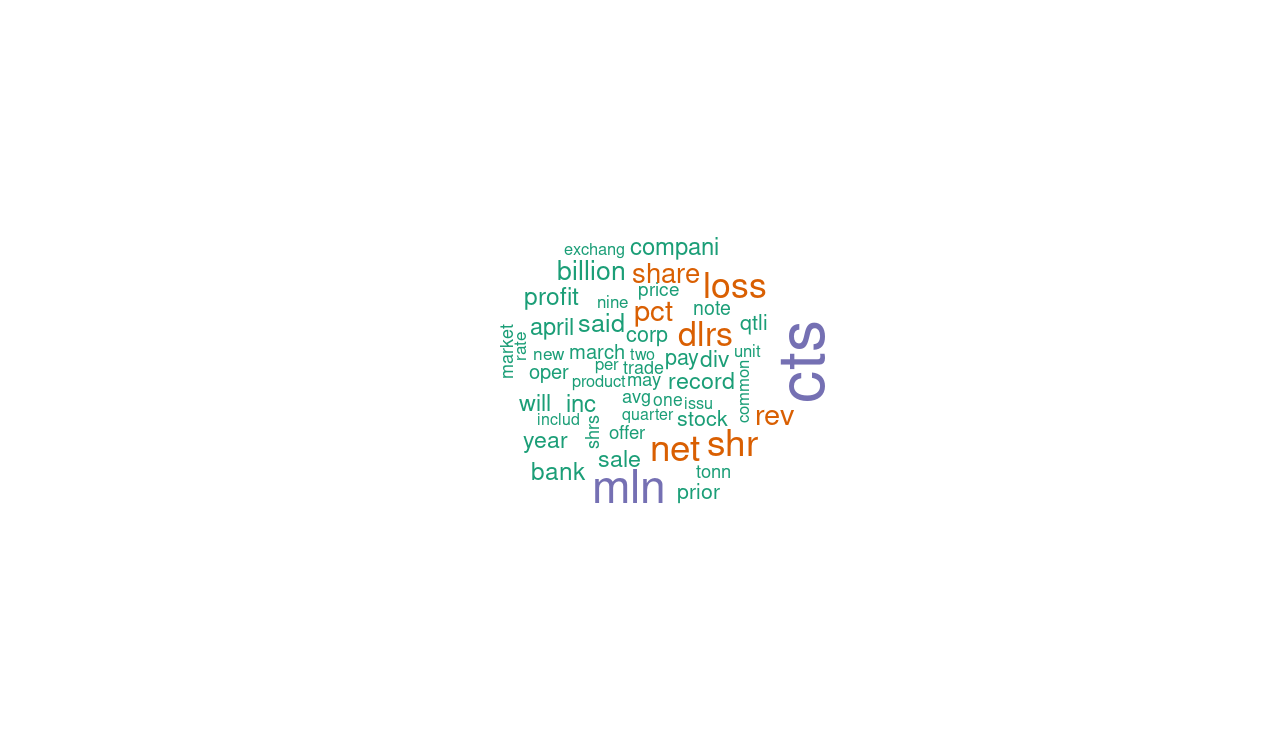
\includegraphics[width=0.8\textwidth]{task2.1.png}
\end{figure}

Draw the word cloud from the TF-IDF document term matrix
\begin{lstlisting}[language=R]
  > bowdtm <- bowdtm[slam::row_sums(bowdtm) > 0, ]
> k <- 20
> result <- LDA(bowdtm, k, method="Gibbs", control=list(iter = 25, verbose = 25, alpha = 0.1))
K = 20; V = 32697; M = 19042
Sampling 25 iterations!
Iteration 25 ...
Gibbs sampling completed!
> result
A LDA_Gibbs topic model with 20 topics.
> terms(result, 10)
      Topic 1   Topic 2   Topic 3   Topic 4    Topic 5   Topic 6   Topic 7   Topic 8      Topic 9    Topic 10  Topic 11  Topic 12  Topic 13  Topic 14 Topic 15 
 [1,] "said"    "said"    "said"    "said"     "dlrs"    "billion" "said"    "tonn"       "bank"     "said"    "said"    "oil"     "said"    "pct"    "said"   
 [2,] "govern"  "will"    "trade"   "trade"    "mln"     "bank"    "market"  "said"       "said"     "share"   "reuter"  "said"    "export"  "will"   "share"  
 [3,] "econom"  "compani" "japan"   "reuter"   "said"    "pct"     "rate"    "mln"        "debt"     "compani" "mine"    "price"   "will"    "issu"   "stock"  
 [4,] "japan"   "new"     "offici"  "futur"    "year"    "franc"   "dollar"  "wheat"      "loan"     "stock"   "gold"    "gas"     "produc"  "said"   "compani"
 [5,] "offici"  "reuter"  "state"   "price"    "quarter" "said"    "bank"    "export"     "billion"  "reuter"  "will"    "barrel"  "price"   "mln"    "inc"    
 [6,] "minist"  "car"     "import"  "pct"      "compani" "year"    "trade"   "reuter"     "dlrs"     "court"   "compani" "product" "coffe"   "bond"   "dlrs"   
 [7,] "year"    "trade"   "japanes" "new"      "sale"    "mln"     "analyst" "agricultur" "will"     "offer"   "ton"     "mln"     "reuter"  "dlrs"   "offer"  
 [8,] "will"    "motor"   "unit"    "cent"     "earn"    "reuter"  "currenc" "year"       "interest" "file"    "oper"    "compani" "meet"    "rate"   "will"   
 [9,] "west"    "exchang" "will"    "tonn"     "share"   "foreign" "dealer"  "grain"      "countri"  "board"   "ounc"    "dlrs"    "countri" "reuter" "reuter" 
[10,] "japanes" "market"  "reuter"  "contract" "report"  "mark"    "exchang" "crop"       "new"      "inc"     "power"   "will"    "quota"   "manag"  "common" 
      Topic 16  Topic 17  Topic 18  Topic 19 Topic 20  
 [1,] "said"    "said"    "said"    "mln"    "pct"     
 [2,] "tax"     "compani" "compani" "cts"    "year"    
 [3,] "billion" "dlrs"    "will"    "net"    "said"    
 [4,] "budget"  "reuter"  "reuter"  "loss"   "billion" 
 [5,] "bill"    "share"   "inc"     "dlrs"   "februari"
 [6,] "stg"     "mln"     "corp"    "shr"    "januari" 
 [7,] "hous"    "corp"    "system"  "reuter" "rose"    
 [8,] "dlrs"    "inc"     "new"     "profit" "rise"    
 [9,] "reuter"  "group"   "servic"  "rev"    "last"    
[10,] "bank"    "will"    "comput"  "oper"   "month"  
\end{lstlisting}

We should remove empty rows in ``bowdtm`` and set number of topics to 20. Then we can compute the LDA model, inferencing via 25 iterations of Gibbs sampling.

We can see the 10 most likely terms within the term probabilities beta of the inferred topics.

We took eight sample documents and get topic proportions form example documents.

\begin{lstlisting}
examples <- c(2, 100, 200, 400, 800, 1000, 1200, 1400)
lapply(pre_process_reuters[examples], as.character)

theta <- tmposterior$topics
N <- length(examples)

tpExamples <- theta[examples,]
colnames(tpExamples) <- nameOfTopics
vizDataFrame <- melt(cbind(data.frame(tpExamples), document = factor(1:N)), variable.name = "topic", id.vars = "document")  
vizDataFrame
\end{lstlisting}

\begin{figure}[H]
  \centering
  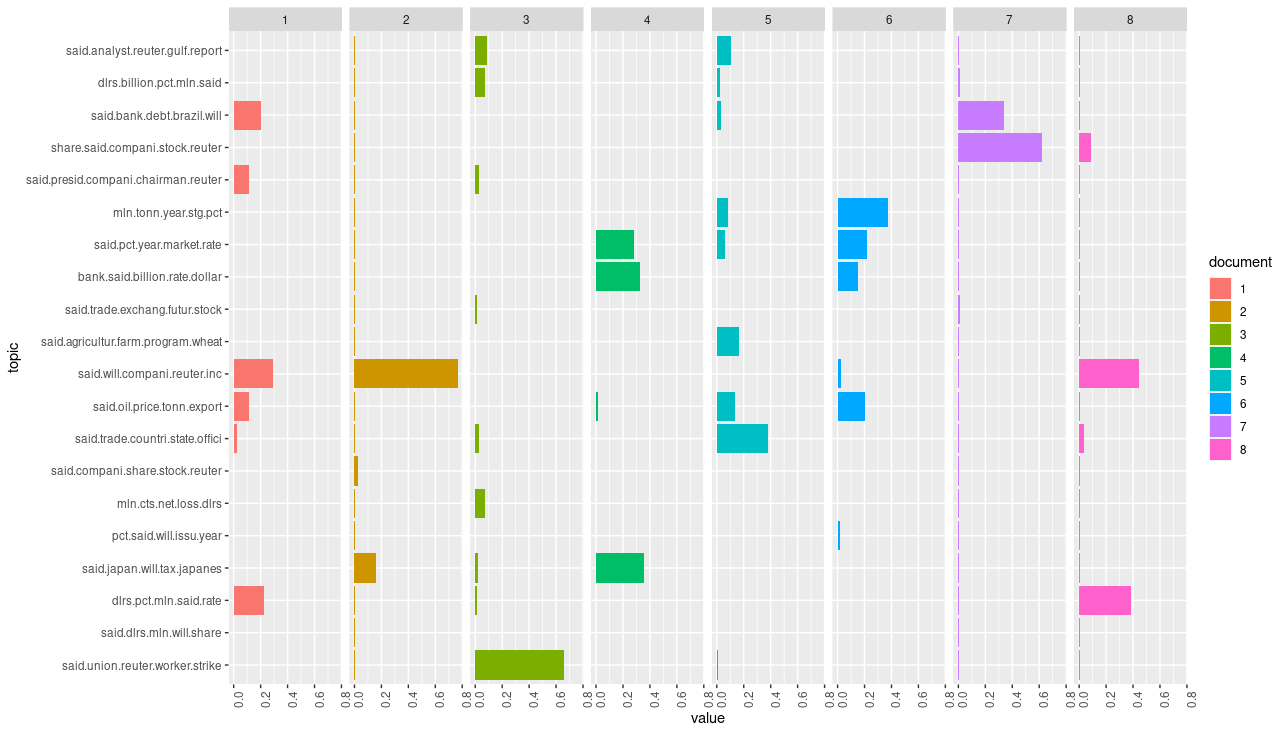
\includegraphics[width=0.8\textwidth]{task2.2.png}
\end{figure}


\section{Task3}
\subsection{Data mining and cleaning}
This data comes from Twitter sentiment analysis in kaggle, From a data set of nearly one million, 13,700 comments about Alan bryd were selected. Among these data, 9,700 positive sentiment data. 4000 negative emotion data. In order to balance the data set, 4000 positive sentiment data and 4000 negative sentiment data were extracted.
 \begin{figure}[H]
\centering
  
\includegraphics[width=1.0\textwidth]{3-1.png} %1.png是图片文件的相对路径

\end{figure}
There are most characters in the comments, such as emoji, @ other users and some garbled characters are inconsistent in capitalization
 \begin{figure}[H]
\centering
  
\includegraphics[width=.8\textwidth]{3-2.png} %1.png是图片文件的相对路径
  \end{figure}
So a series of data cleaning operations are used to clean the data.
 \begin{figure}[H]
\centering
  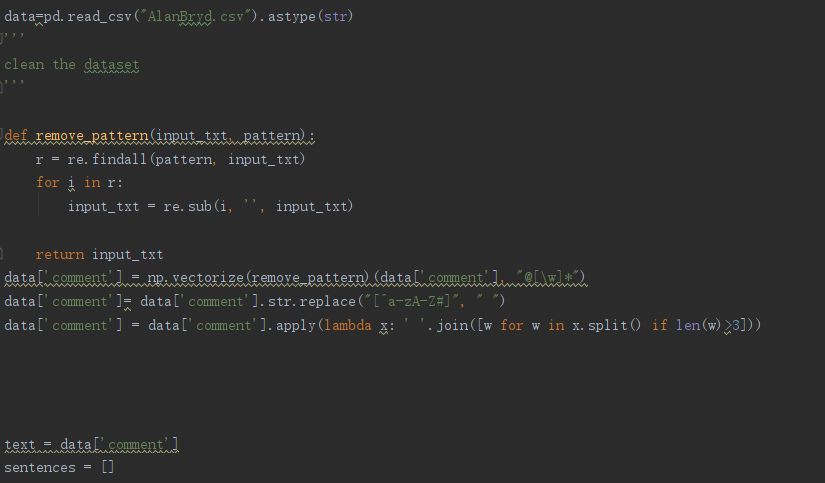
\includegraphics[width=.8\textwidth]{3-3.png} %1.png是图片文件的相对路径
  \end{figure}
\subsection{Use word2vec to build word vectors}
 \begin{figure}[H]
\centering
  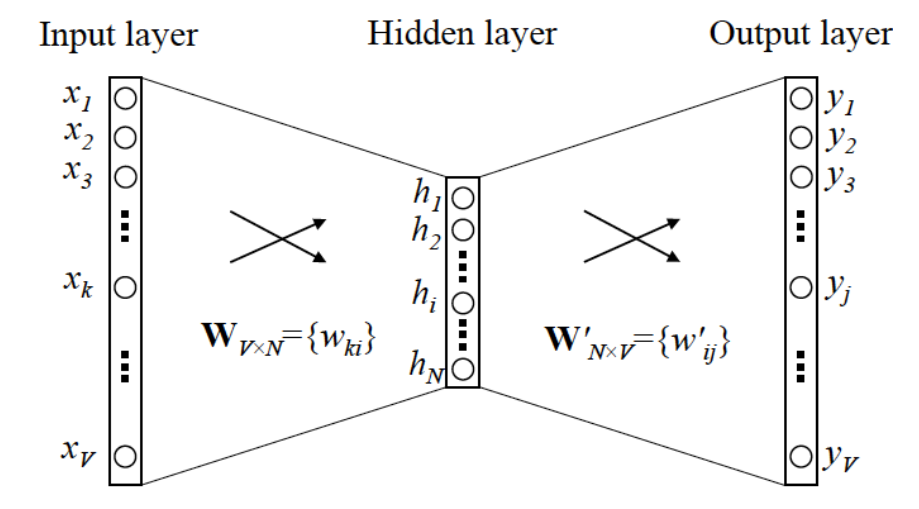
\includegraphics[width=.8\textwidth]{3-4.png} %1.png是图片文件的相对路径
  \end{figure}
Use word2vec's word vector for word embedding as input to the model
 \begin{figure}[H]
\centering
  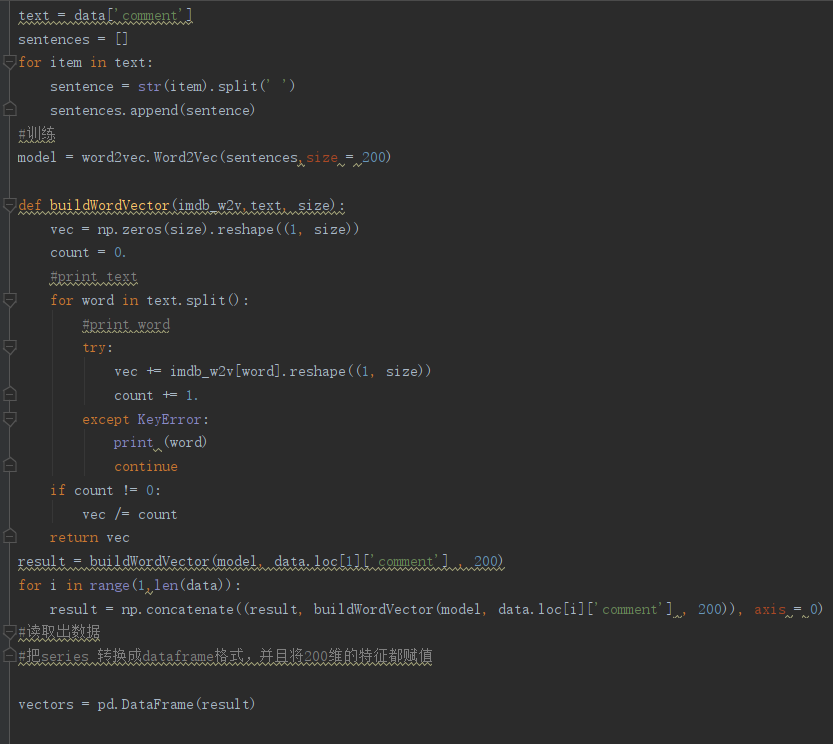
\includegraphics[width=.8\textwidth]{3-5.png} %1.png是图片文件的相对路径
  \end{figure}
\subsection{model using and result}
\subsubsection{GBDT}
theory of GBDT
 \begin{figure}[H]
\centering
  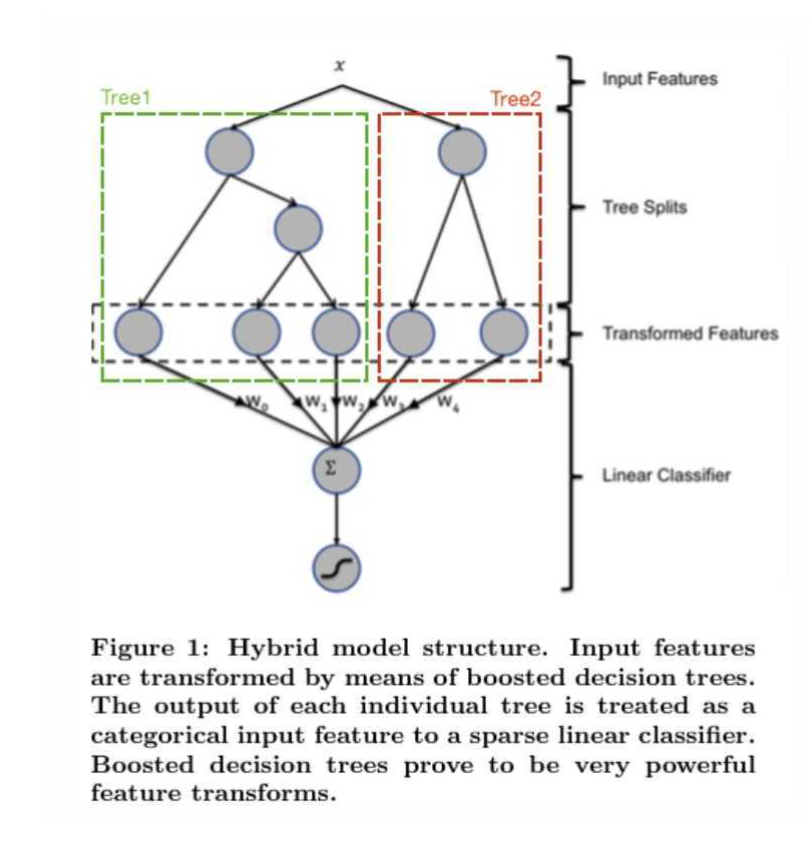
\includegraphics[width=.8\textwidth]{3-6.png} %1.png是图片文件的相对路径
  \end{figure}
Parameters of gbdt:\\
    $n_estimators=1000,$
    $subsample=0.8,$
    $loss='deviance',$
    $max_features='sqrt',$

  \subsubsection{SVM}
 theory of SVM
  \begin{figure}[H]
\centering
  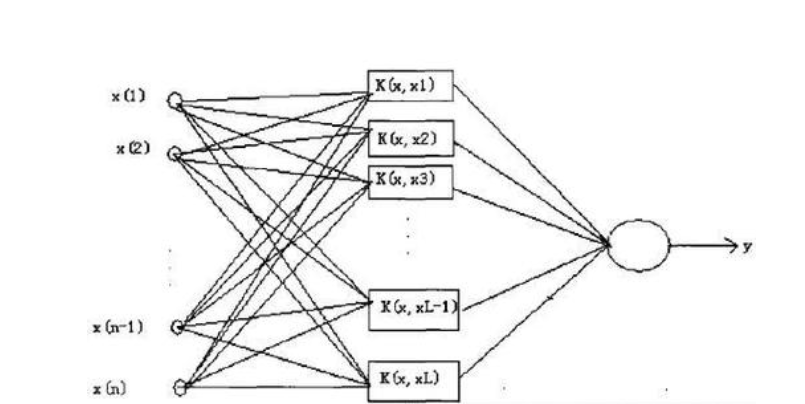
\includegraphics[width=.8\textwidth]{3-7.png} %1.png是图片文件的相对路径
  \end{figure}
Parameters of SVM:
$
kernel=‘rbf’
degree=3
$
\subsubsection{RandomForest}
 theory of RF
   \begin{figure}[H]
\centering
  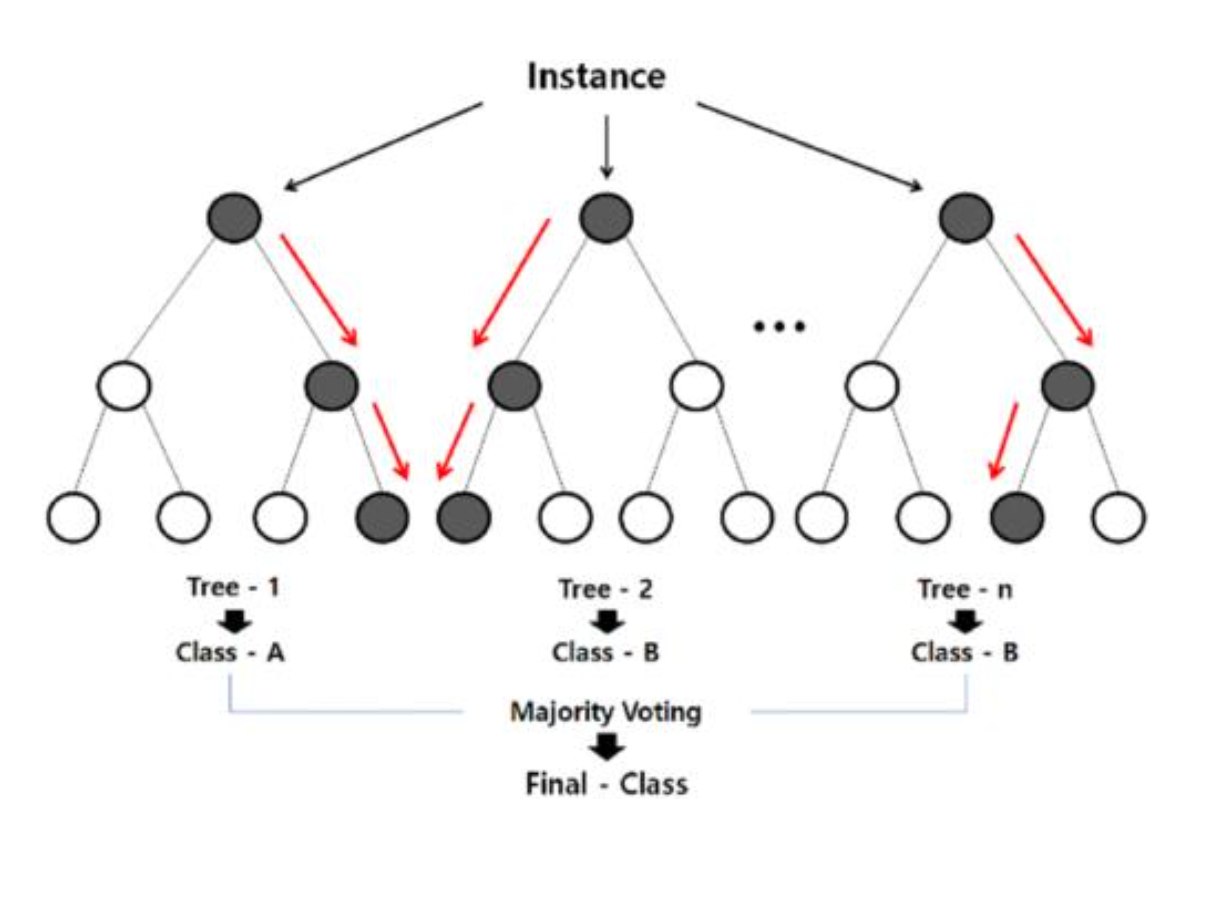
\includegraphics[width=.8\textwidth]{3-8.png} %1.png是图片文件的相对路径
  \end{figure}
Parameters of RF:$
    oob_score=True,
    n_estimators=400,
    max_features='sqrt',
    $
\subsubsection{ExtraTrees}
theory of ET
   \begin{figure}[H]
\centering
  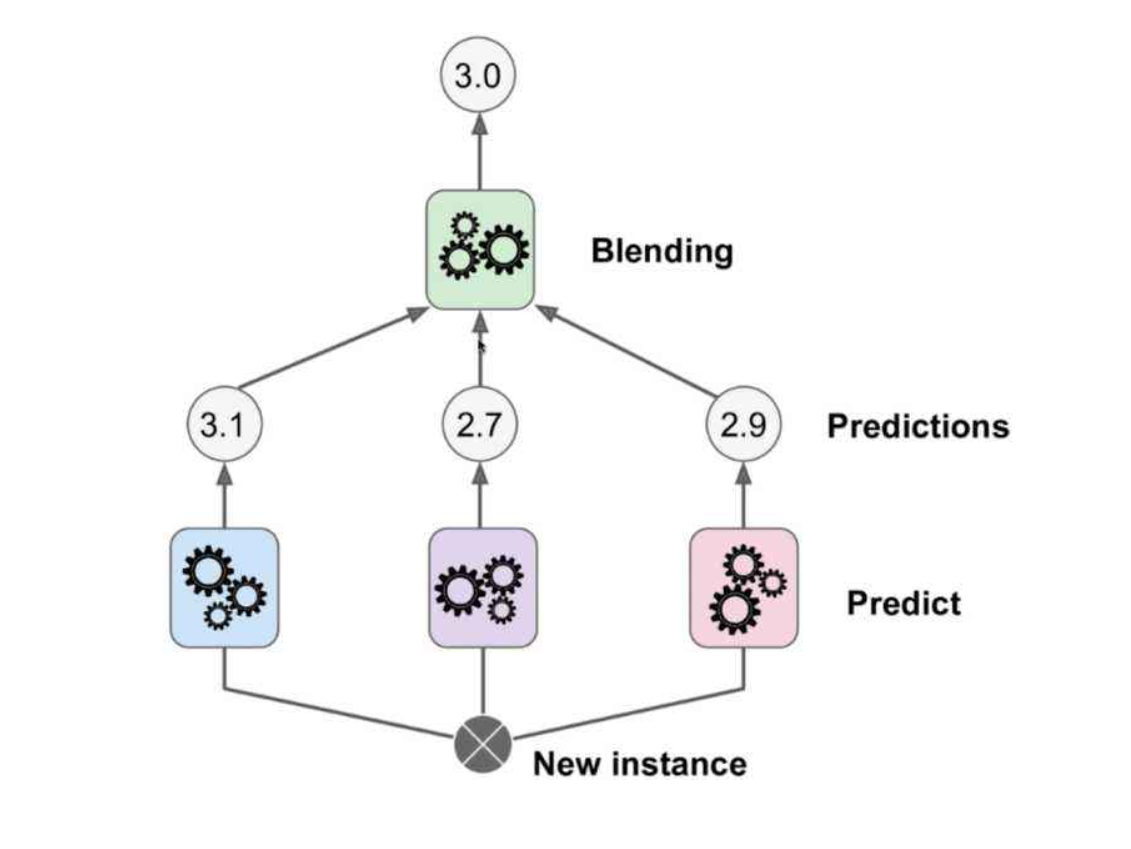
\includegraphics[width=.8\textwidth]{3-9.png} %1.png是图片文件的相对路径
  \end{figure}
 Parameter of ET:
 $
 criterion=gini,
 max features=log,
 max depth=50
 $
 \subsubsection{Result}
    \begin{figure}[H]
\centering
  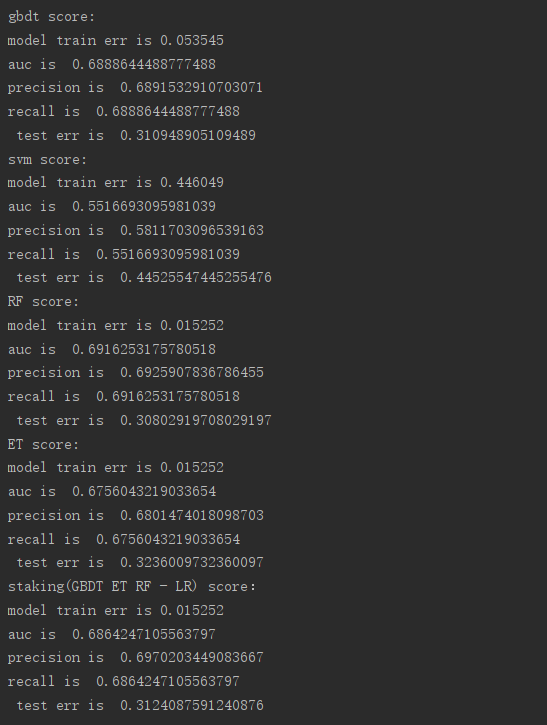
\includegraphics[width=.8\textwidth]{3-10.png} %1.png是图片文件的相对路径
  \end{figure}
According to the picture above,The expressive power of gbdt is better than other models in all aspects, and the mathematical model in machine learning can fit the features well when the data set is not large. Compared with other tree models, GBDT has a stronger ability to fit data by calculating residuals.
The auc figure of GBDT is :
    \begin{figure}[H]
\centering
  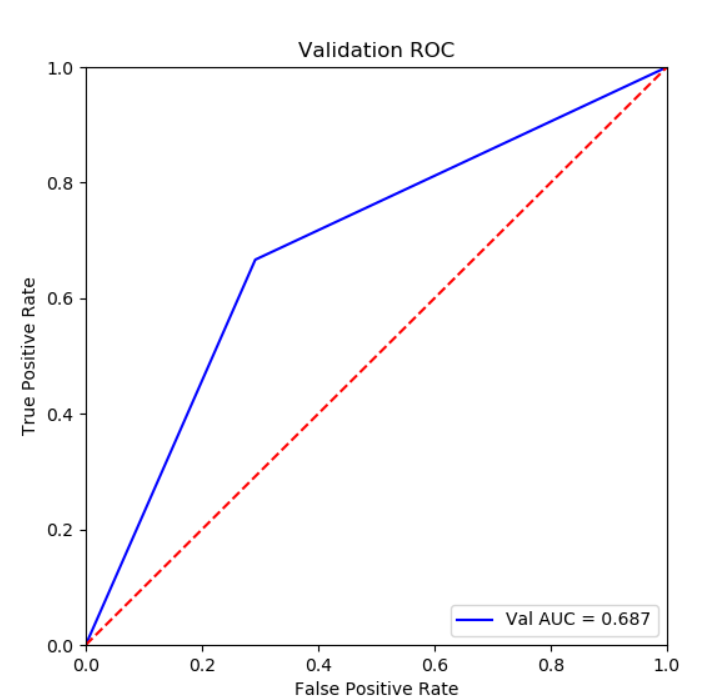
\includegraphics[width=.8\textwidth]{3-11.png} %1.png是图片文件的相对路径
  \end{figure}

\section{contribution}
Wangzhihui Mei: $25\%$ \\
Hongyi Huang: $25\%$ \\
Chang Xu: $25\%$ \\
Zijia He: $25\%$
\end{document}
